% This is "sig-alternate.tex" V2.0 May 2012
% This file should be compiled with V2.5 of "sig-alternate.cls" May 2012
%
% This example file demonstrates the use of the 'sig-alternate.cls'
% V2.5 LaTeX2e document class file. It is for those submitting
% articles to ACM Conference Proceedings WHO DO NOT WISH TO
% STRICTLY ADHERE TO THE SIGS (PUBS-BOARD-ENDORSED) STYLE.
% The 'sig-alternate.cls' file will produce a similar-looking,
% albeit, 'tighter' paper resulting in, invariably, fewer pages.
%
% ----------------------------------------------------------------------------------------------------------------
% This .tex file (and associated .cls V2.5) produces:
%       1) The Permission Statement
%       2) The Conference (location) Info information
%       3) The Copyright Line with ACM data
%       4) NO page numbers
%
% as against the acm_proc_article-sp.cls file which
% DOES NOT produce 1) thru' 3) above.
%
% Using 'sig-alternate.cls' you have control, however, from within
% the source .tex file, over both the CopyrightYear
% (defaulted to 200X) and the ACM Copyright Data
% (defaulted to X-XXXXX-XX-X/XX/XX).
% e.g.
% \CopyrightYear{2007} will cause 2007 to appear in the copyright line.
% \crdata{0-12345-67-8/90/12} will cause 0-12345-67-8/90/12 to appear in the copyright line.
%
% ---------------------------------------------------------------------------------------------------------------
% This .tex source is an example which *does* use
% the .bib file (from which the .bbl file % is produced).
% REMEMBER HOWEVER: After having produced the .bbl file,
% and prior to final submission, you *NEED* to 'insert'
% your .bbl file into your source .tex file so as to provide
% ONE 'self-contained' source file.
%
% ================= IF YOU HAVE QUESTIONS =======================
% Questions regarding the SIGS styles, SIGS policies and
% procedures, Conferences etc. should be sent to
% Adrienne Griscti (griscti@acm.org)
%
% Technical questions _only_ to
% Gerald Murray (murray@hq.acm.org)
% ===============================================================
%
% For tracking purposes - this is V2.0 - May 2012

\documentclass{sig-alternate-2013}

\newfont{\mycrnotice}{ptmr8t at 7pt}
\newfont{\myconfname}{ptmri8t at 7pt}
\let\crnotice\mycrnotice%
\let\confname\myconfname%

%\permission{Permission to make digital or hard copies of part or all of this work for personal or classroom use is granted without fee provided that copies are not made or distributed for profit or commercial advantage, and that copies bear this notice and the full citation on the first page. Copyrights for third-party components of this work must be honored. For all other uses, contact the owner/author(s). Copyright is held by the author/owner(s).}
%\conferenceinfo{HRI'14,}{March 3--6, 2014, Bielefeld, Germany.} 
%\copyrightetc{ACM \the\acmcopyr}
%\crdata{978-1-4503-2658-2/14/03. \\
%http://dx.doi.org/10.1145/2559636.2559816}

\clubpenalty=10000 
\widowpenalty = 10000

\graphicspath{{./img/}}
\begin{document}

\title{The title of your paper} % or sth. like that
%\titlenote{A full version of this paper is available as
%\textit{Author's Guide to Preparing ACM SIG Proceedings Using
%\LaTeX$2_\epsilon$\ and BibTeX} at
%\texttt{www.acm.org/eaddress.htm}}}
%
% You need the command \numberofauthors to handle the 'placement
% and alignment' of the authors beneath the title.
%
% For aesthetic reasons, we recommend 'three authors at a time'
% i.e. three 'name/affiliation blocks' be placed beneath the title.
%
% NOTE: You are NOT restricted in how many 'rows' of
% "name/affiliations" may appear. We just ask that you restrict
% the number of 'columns' to three.
%
% Because of the available 'opening page real-estate'
% we ask you to refrain from putting more than six authors
% (two rows with three columns) beneath the article title.
% More than six makes the first-page appear very cluttered indeed.
%
% Use the \alignauthor commands to handle the names
% and affiliations for an 'aesthetic maximum' of six authors.
% Add names, affiliations, addresses for
% the seventh etc. author(s) as the argument for the
% \additionalauthors command.
% These 'additional authors' will be output/set for you
% without further effort on your part as the last section in
% the body of your article BEFORE References or any Appendices.

\numberofauthors{2} %  in this sample file, there are a *total*
% of EIGHT authors. SIX appear on the 'first-page' (for formatting
% reasons) and the remaining two appear in the \additionalauthors section.
%
\author{
% You can go ahead and credit any number of authors here,
% e.g. one 'row of three' or two rows (consisting of one row of three
% and a second row of one, two or three).
%
% The command \alignauthor (no curly braces needed) should
% precede each author name, affiliation/snail-mail address and
% e-mail address. Additionally, tag each line of
% affiliation/address with \affaddr, and tag the
% e-mail address with \email.
%
% 1st. author
\alignauthor Ivana Kaji\'c\\
       \affaddr{Bernstein Center for Computational Neuroscience}\\
       \affaddr{Berlin, Germany}
       %\email{hafner@informatik.hu-berlin.de}     
\alignauthor Other Authors\\
       \affaddr{Department of Computer Science}
       \affaddr{Berlin, Germany}
       %\email{hafner@informatik.hu-berlin.de}
}
% There's nothing stopping you putting the seventh, eighth, etc.
% author on the opening page (as the 'third row') but we ask,
% for aesthetic reasons that you place these 'additional authors'
% in the \additional authors block, viz.

\maketitle
\begin{abstract}
Hand-eye coordination is an important motor skill acquired in infancy which precedes pointing behavior. Pointing facilitates social interactions by directing attention of engaged participants. It is thus essential for the natural flow of human-robot interaction. Here, we attempt to explain how pointing emerges from sensorimotor learning of hand-eye coordination in a humanoid robot. During a body babbling phase with a random walk strategy, a robot learned mappings of joints for different arm postures. Arm joint configurations were used to train biologically inspired models consisting of SOMs. We show that such a model implemented on a robotic platform accounts for pointing behavior while humans present objects out of reach of the robot's hand.
\end{abstract}

% A category with the (minimum) three required fields
%\category{H.4}{Information Systems Applications}{Miscellaneous}
%A category including the fourth, optional field follows...
%\category{D.2.8}{Software Engineering}{Metrics}[complexity measures, performance measures]

%\terms{Theory}

\keywords{cognitive robotics, HRI, sensorimotor coupling}

\section{Introduction}
Hand-eye coordination is an important motor skill acquired in infancy which precedes pointing behavior. Pointing facilitates social interactions by directing attention of engaged participants. It is thus essential for the natural flow of human-robot interaction. Here, we attempt to explain how pointing emerges from sensorimotor learning of hand-eye coordination in a humanoid robot. During a body babbling phase with a random walk strategy, a robot learned mappings of joints for different arm postures. Arm joint configurations were used to train biologically inspired models consisting of SOMs. We show that such a model implemented on a robotic platform accounts for pointing behavior while humans present objects out of reach of the robot's hand.
\cite{Hafner2011}
\section{Biologically inspired model}
Hand-eye coordination is an important motor skill acquired in infancy which precedes pointing behavior. Pointing facilitates social interactions by directing attention of engaged participants. It is thus essential for the natural flow of human-robot interaction. Here, we attempt to explain how pointing emerges from sensorimotor learning of hand-eye coordination in a humanoid robot. During a body babbling phase with a random walk strategy, a robot learned mappings of joints for different arm postures. Arm joint configurations were used to train biologically inspired models consisting of SOMs. We show that such a model implemented on a robotic platform accounts for pointing behavior while humans present objects out of reach of the robot's hand.

\section{Results}
Hand-eye coordination is an important motor skill acquired in infancy which precedes pointing behavior. Pointing facilitates social interactions by directing attention of engaged participants. It is thus essential for the natural flow of human-robot interaction. Here, we attempt to explain how pointing emerges from sensorimotor learning of hand-eye coordination in a humanoid robot. During a body babbling phase with a random walk strategy, a robot learned mappings of joints for different arm postures. Arm joint configurations were used to train biologically inspired models consisting of SOMs. We show that such a model implemented on a robotic platform accounts for pointing behavior while humans present objects out of reach of the robot's hand.
\begin{figure}
\centering
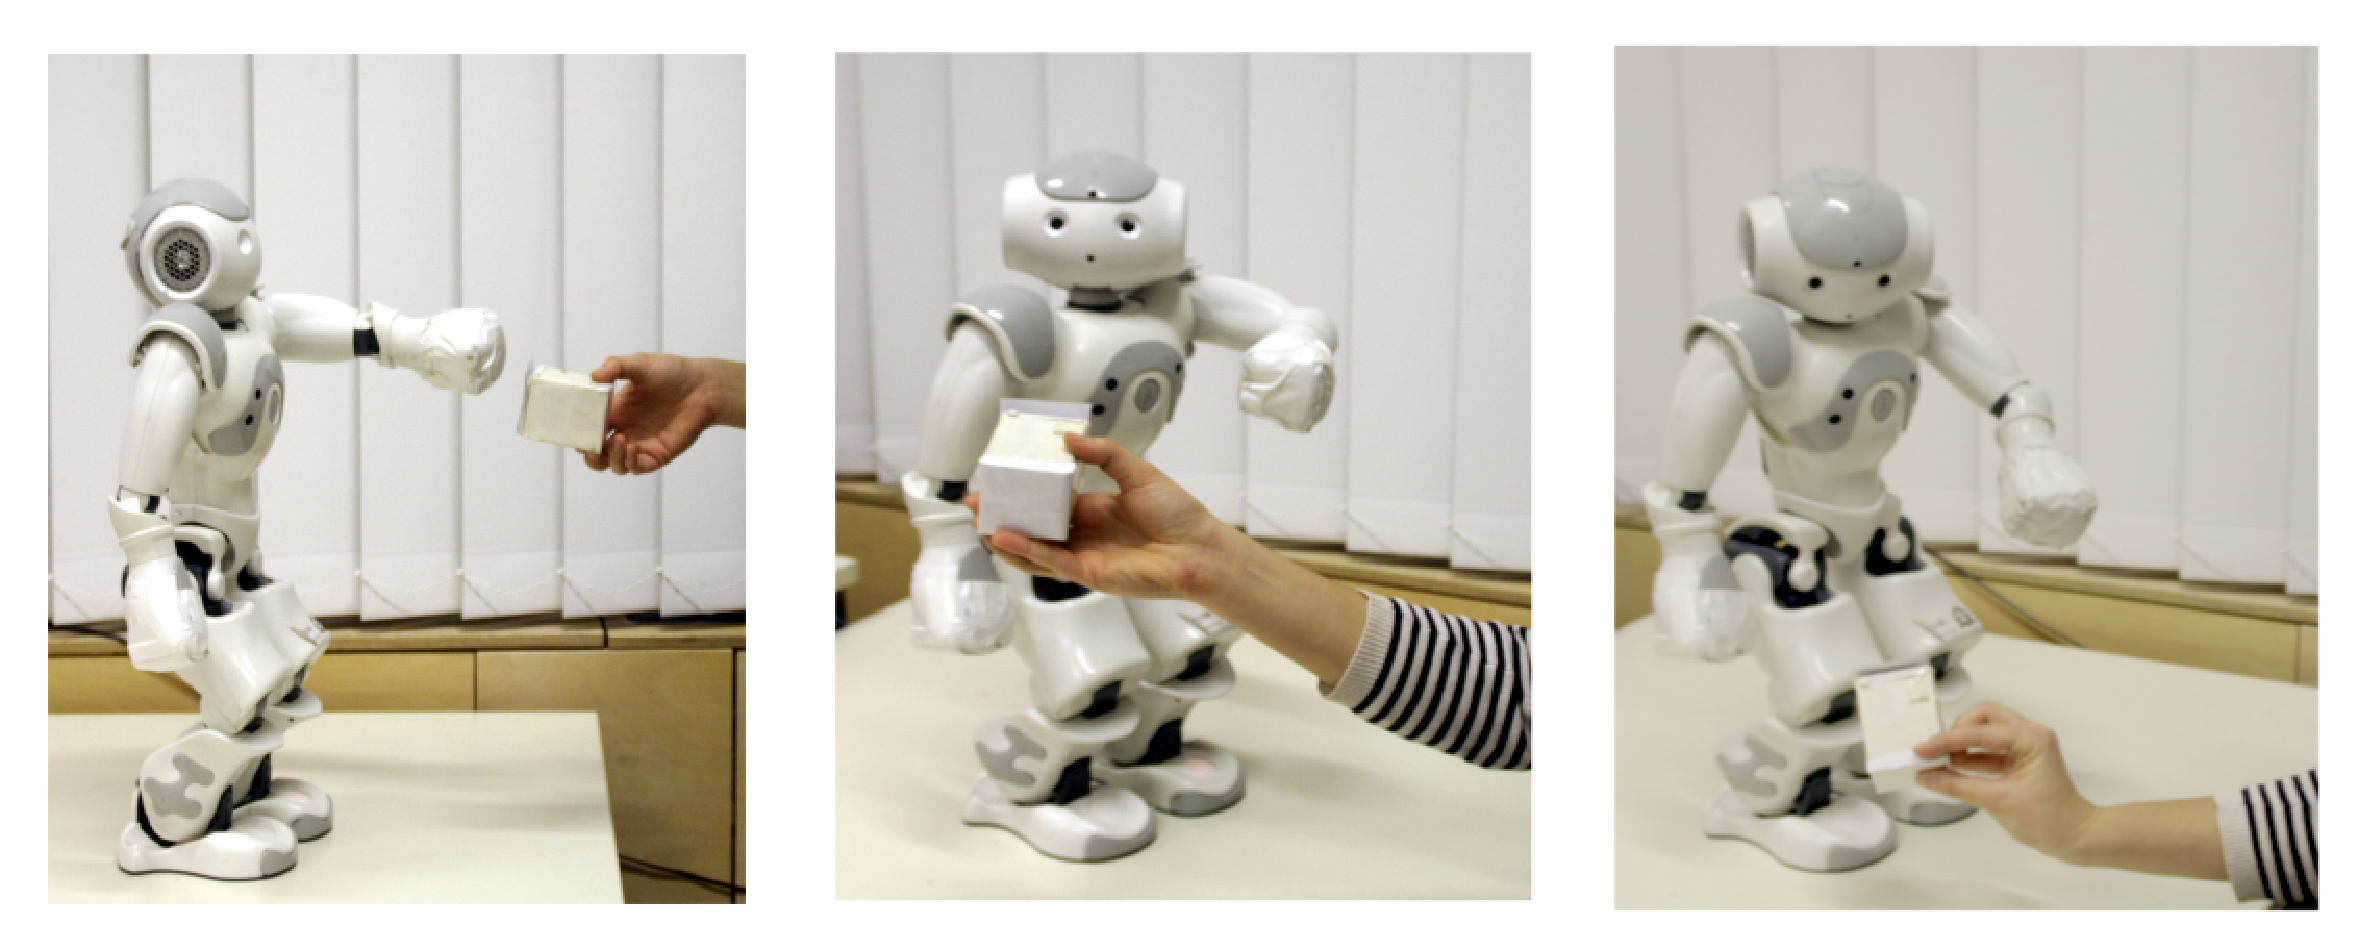
\includegraphics[height=3.5cm]{experiment.eps}
\caption{Human-robot interaction}
\label{lab:experiment}
\end{figure}


\section{Future work}
...

%ACKNOWLEDGMENTS are optional

\section{Acknowledgments}
Thanks!

%
% The following two commands are all you need in the
% initial runs of your .tex file to
% produce the bibliography for the citations in your paper.
\bibliographystyle{abbrv}
\bibliography{sigproc}  % sigproc.bib is the name of the Bibliography in this case
% You must have a proper ".bib" file
%  and remember to run:
% latex bibtex latex latex
% to resolve all references
%
% ACM needs 'a single self-contained file'!
%
%APPENDICES are optional
%\balancecolumns

\end{document}